\documentclass[amsmath, amssymb,
%twocolumn,
%linenumbers,
nobibnotes, superscriptaddress]{revtex4-1}
\usepackage{graphicx}
\usepackage{dcolumn}   % needed for some tables
\usepackage{hyperref}
\usepackage{epstopdf}
\usepackage{multirow}
\usepackage{subfigure}
\usepackage{longtable}
%\usepackage{floatfix}
\usepackage{float}

\usepackage{color}
\definecolor{darkblue}{rgb}{0,0,0.5}

\usepackage{hyperref}  % Create clickable links for figures, tables, and references. Work only with pdflatex
\hypersetup{
    colorlinks=true, %set true if you want colored links
%    linktoc=all,     %set to all if you want both sections and subsections linked
    linkcolor=darkblue,  %choose some color if you want links to stand out
    urlcolor=darkblue,
    citecolor=darkblue,
    filecolor=darkblue,
}

\setlength{\textheight}{9.5in}

\begin{document}

%%highpt

\begin{figure}[H] 
\begin{center}
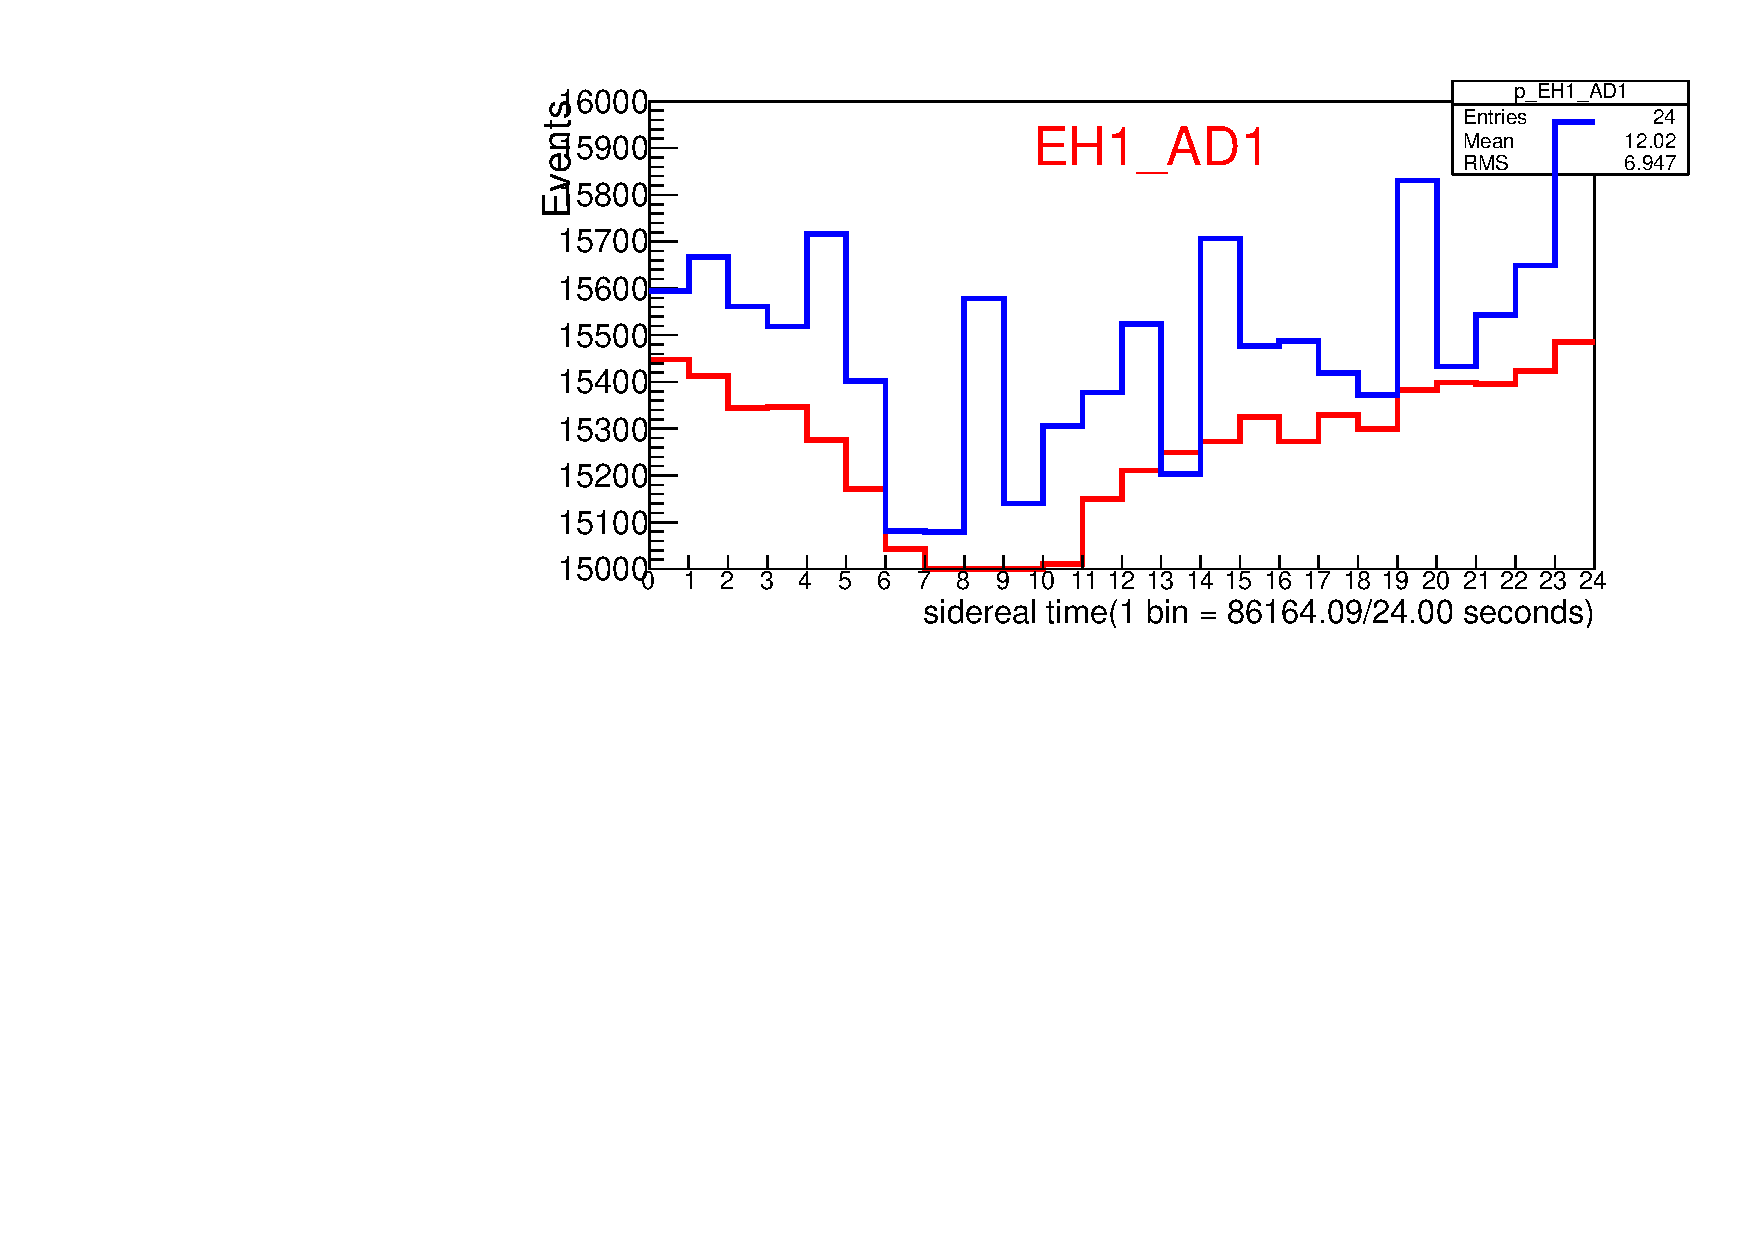
\includegraphics[width=6cm]{MeasurementPredictionEH1_AD1.pdf}
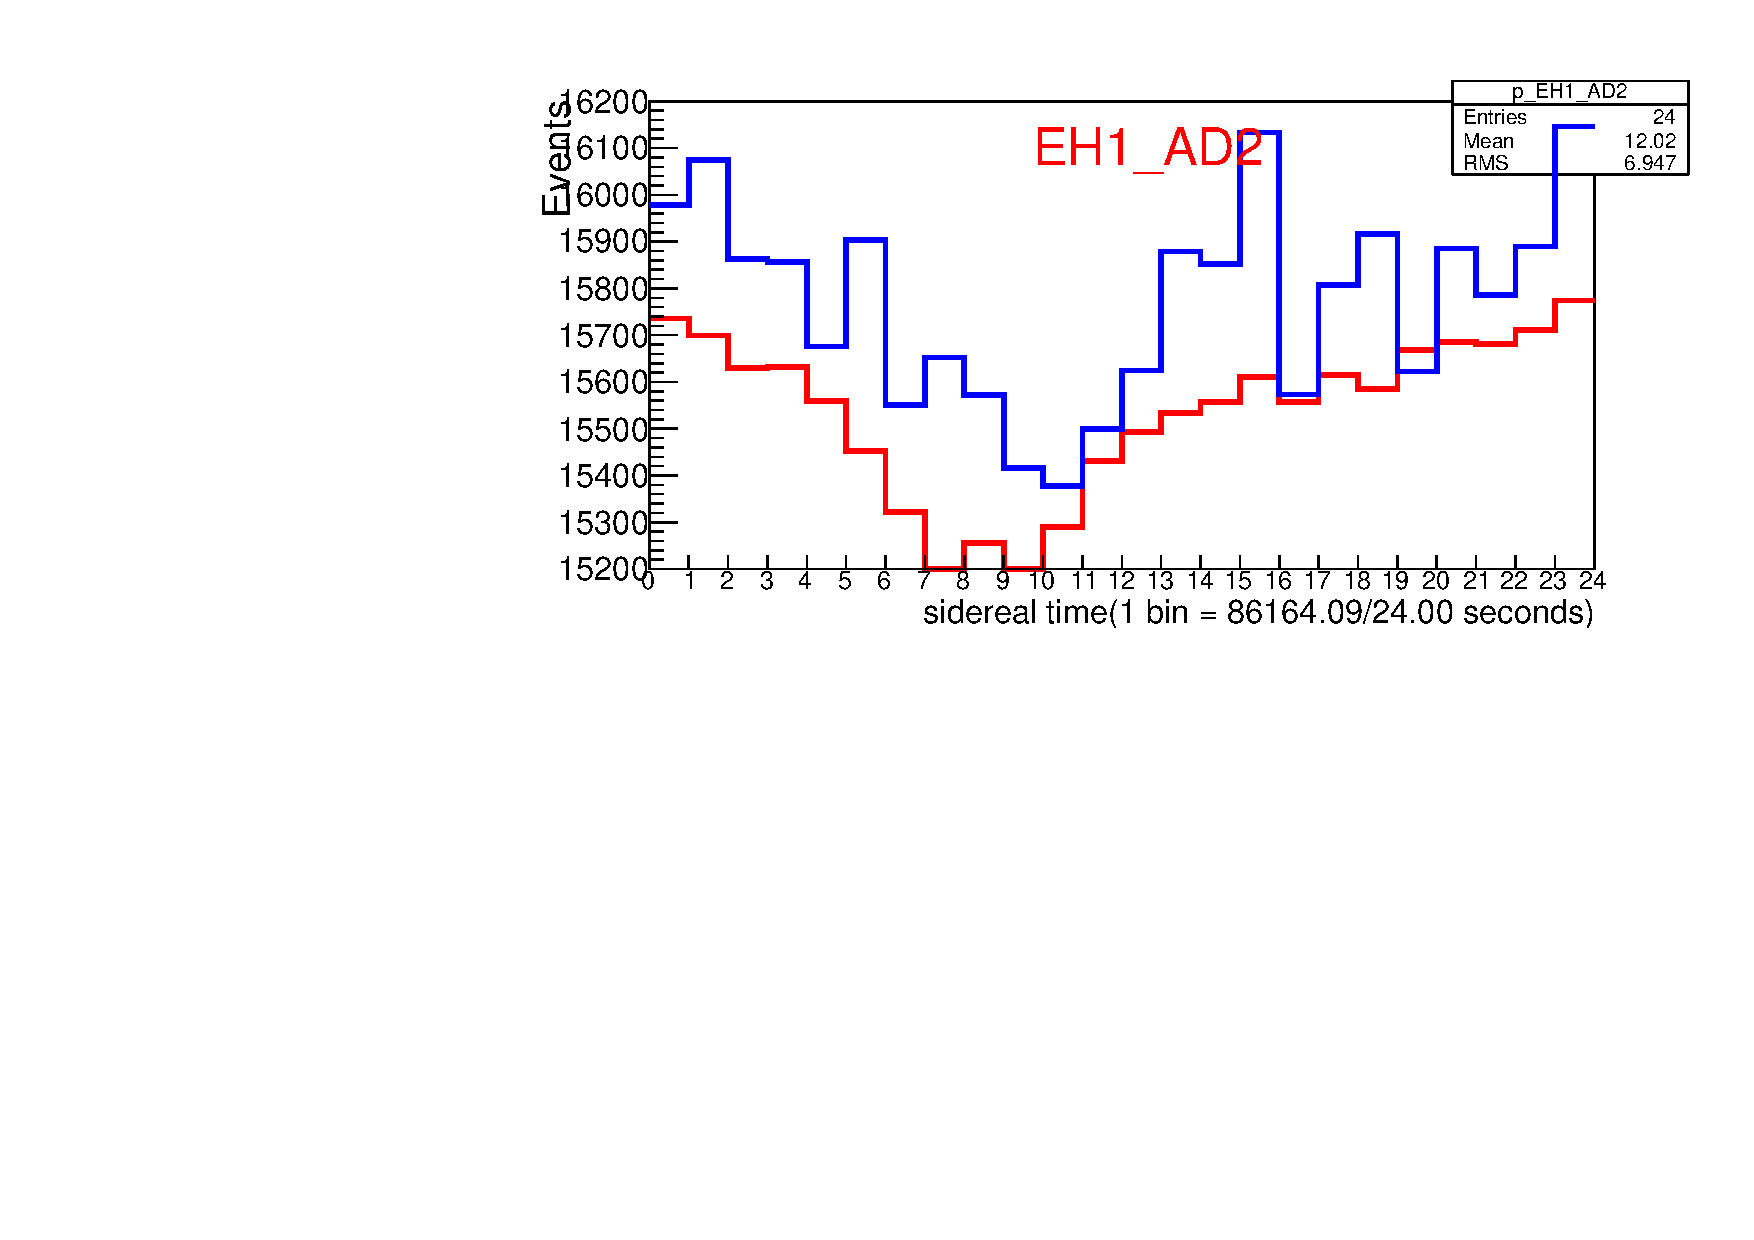
\includegraphics[width=6cm]{MeasurementPredictionEH1_AD2.pdf}\\
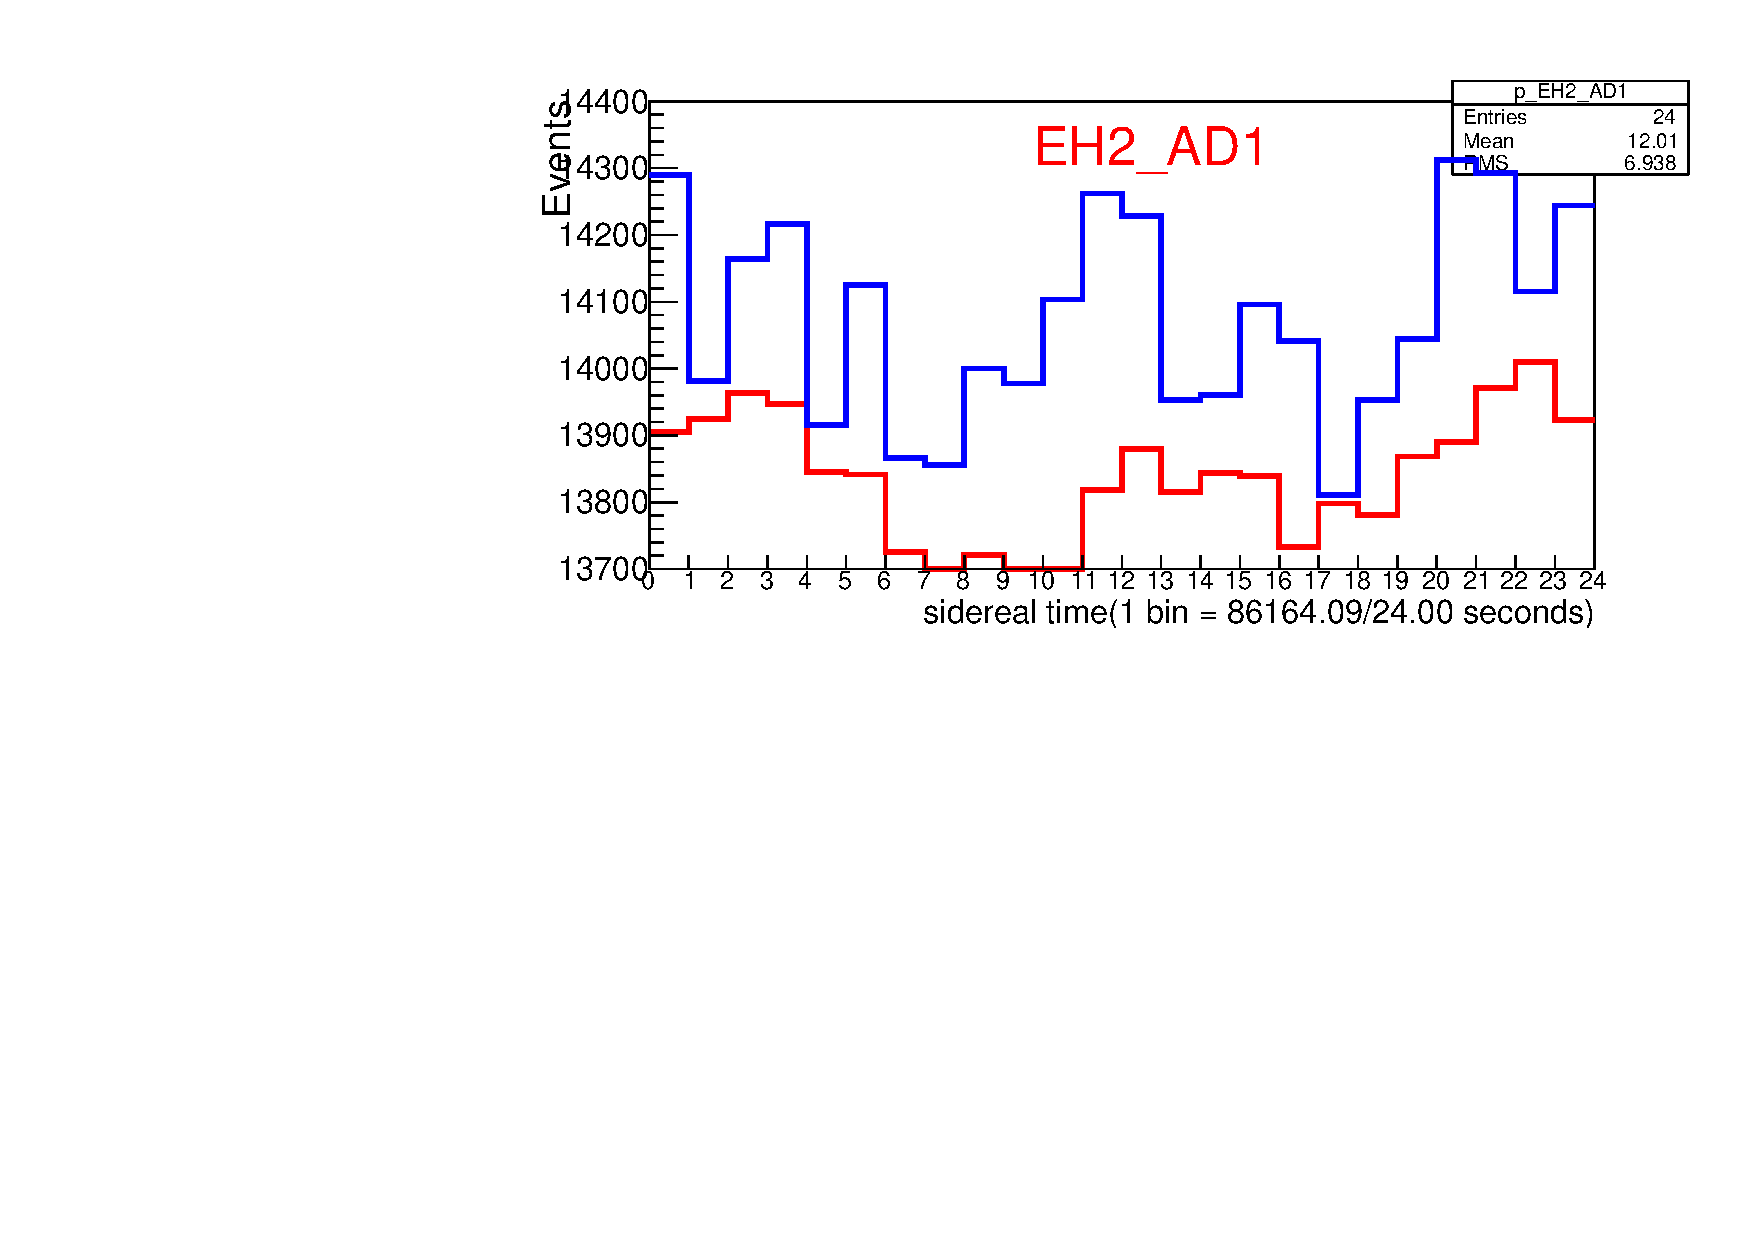
\includegraphics[width=6cm]{MeasurementPredictionEH2_AD1.pdf}
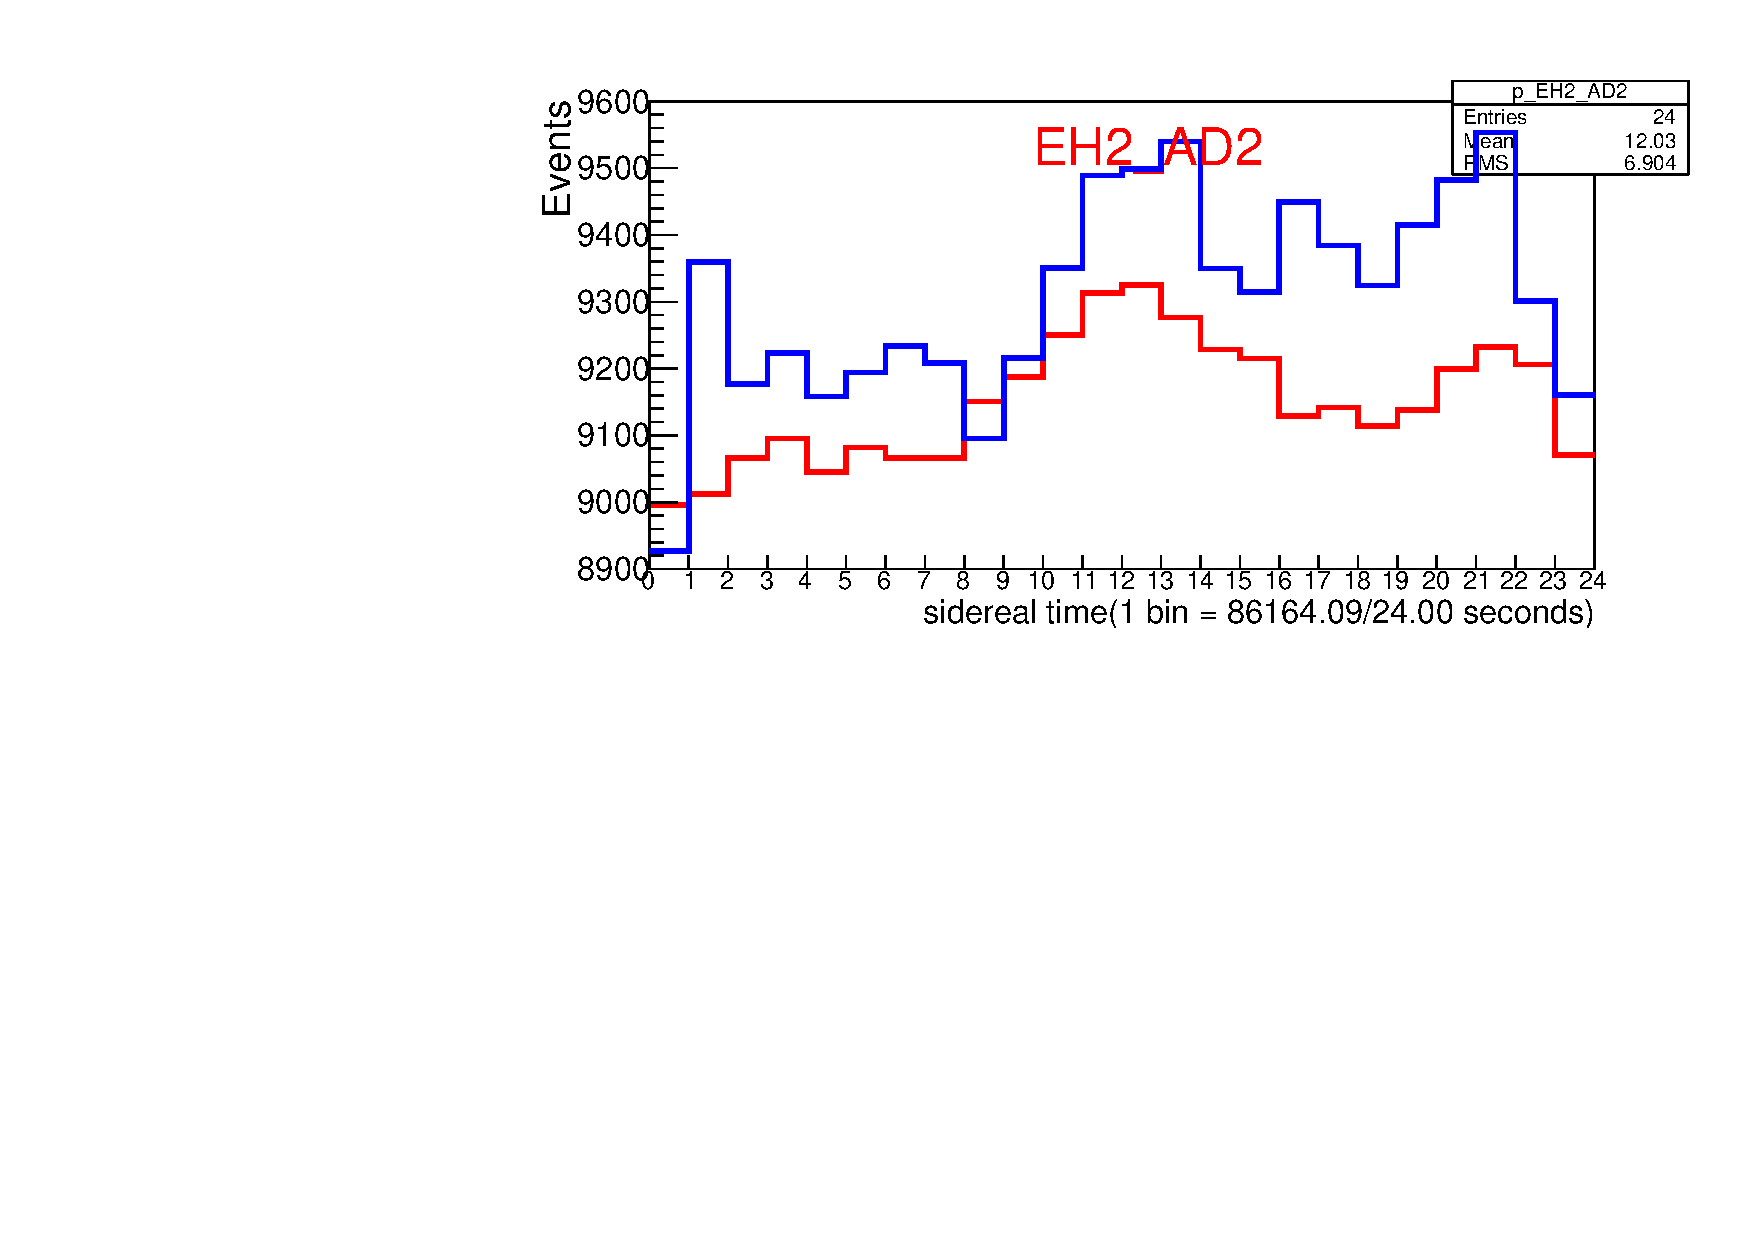
\includegraphics[width=6cm]{MeasurementPredictionEH2_AD2.pdf}\\
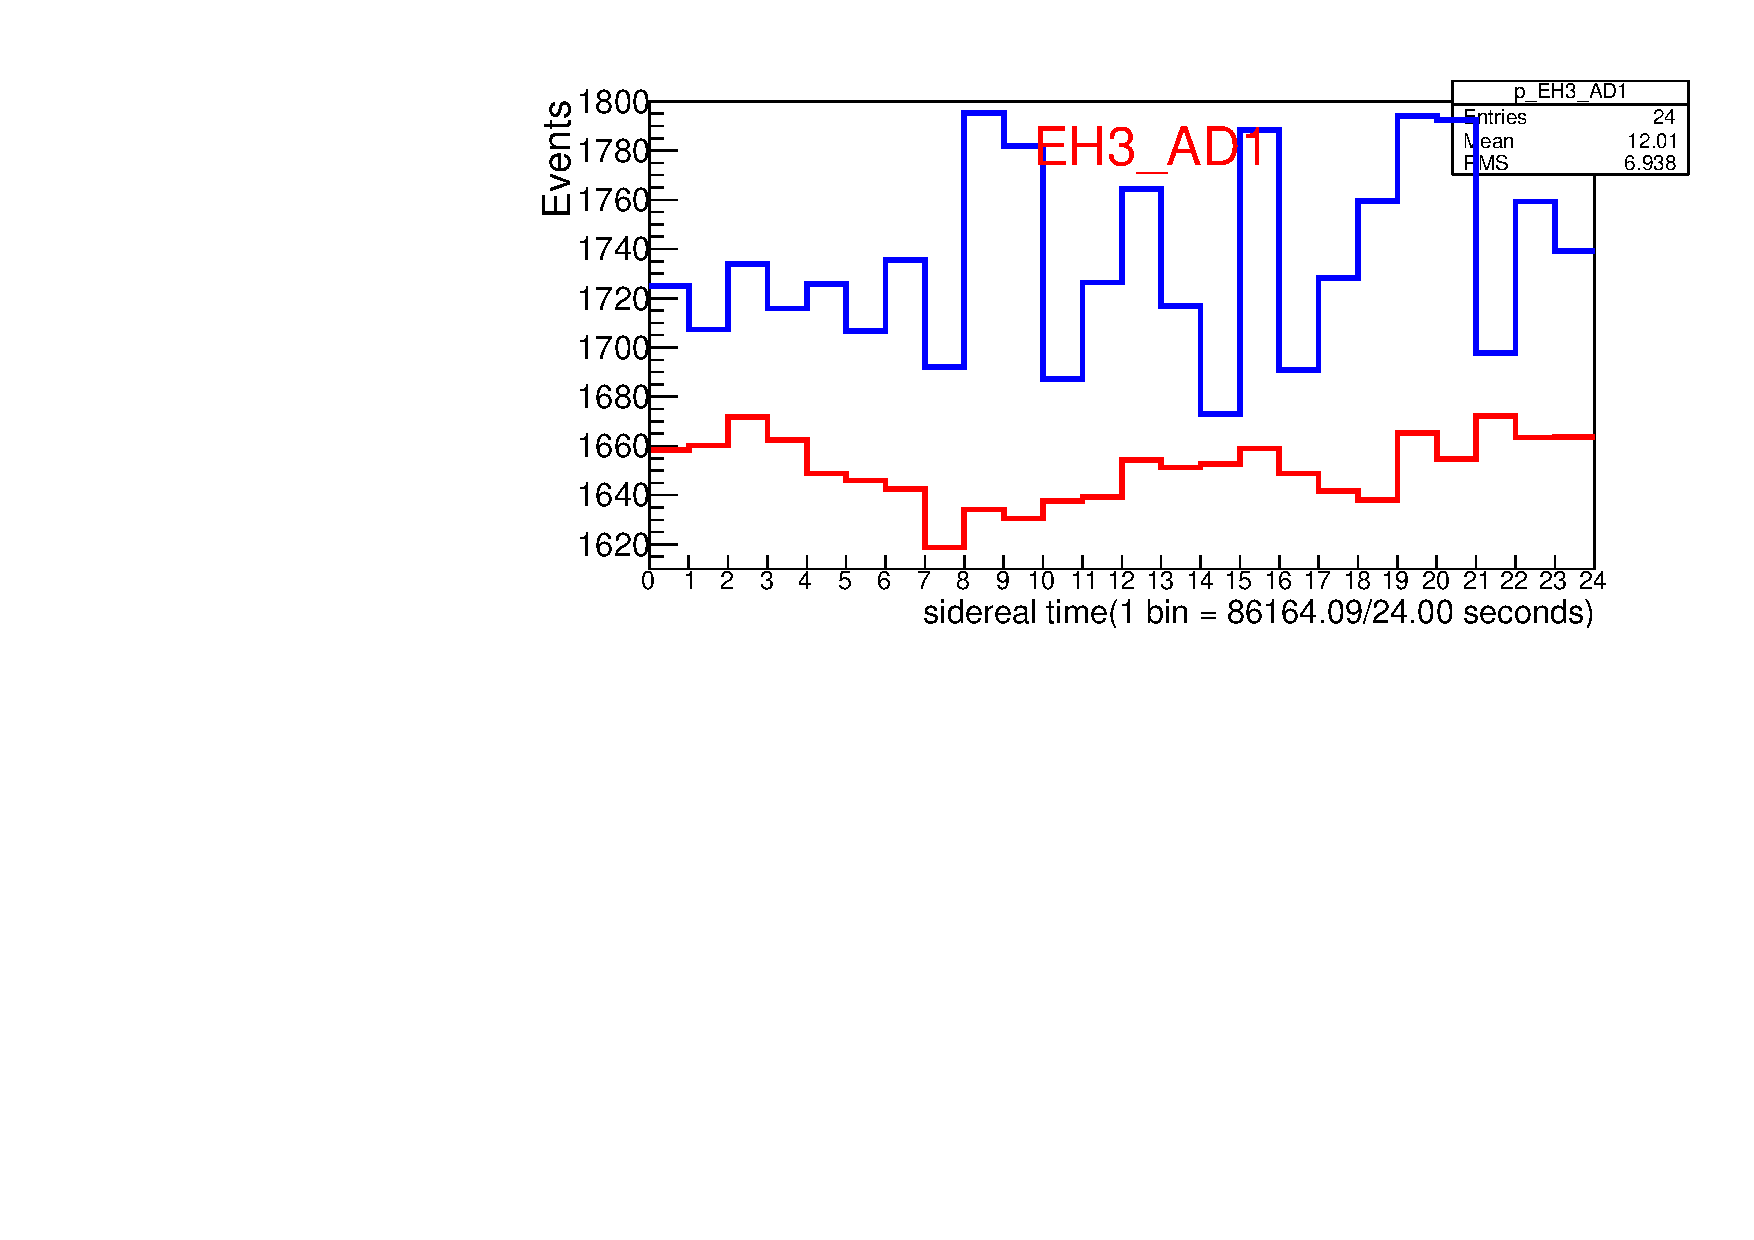
\includegraphics[width=6cm]{MeasurementPredictionEH3_AD1.pdf}
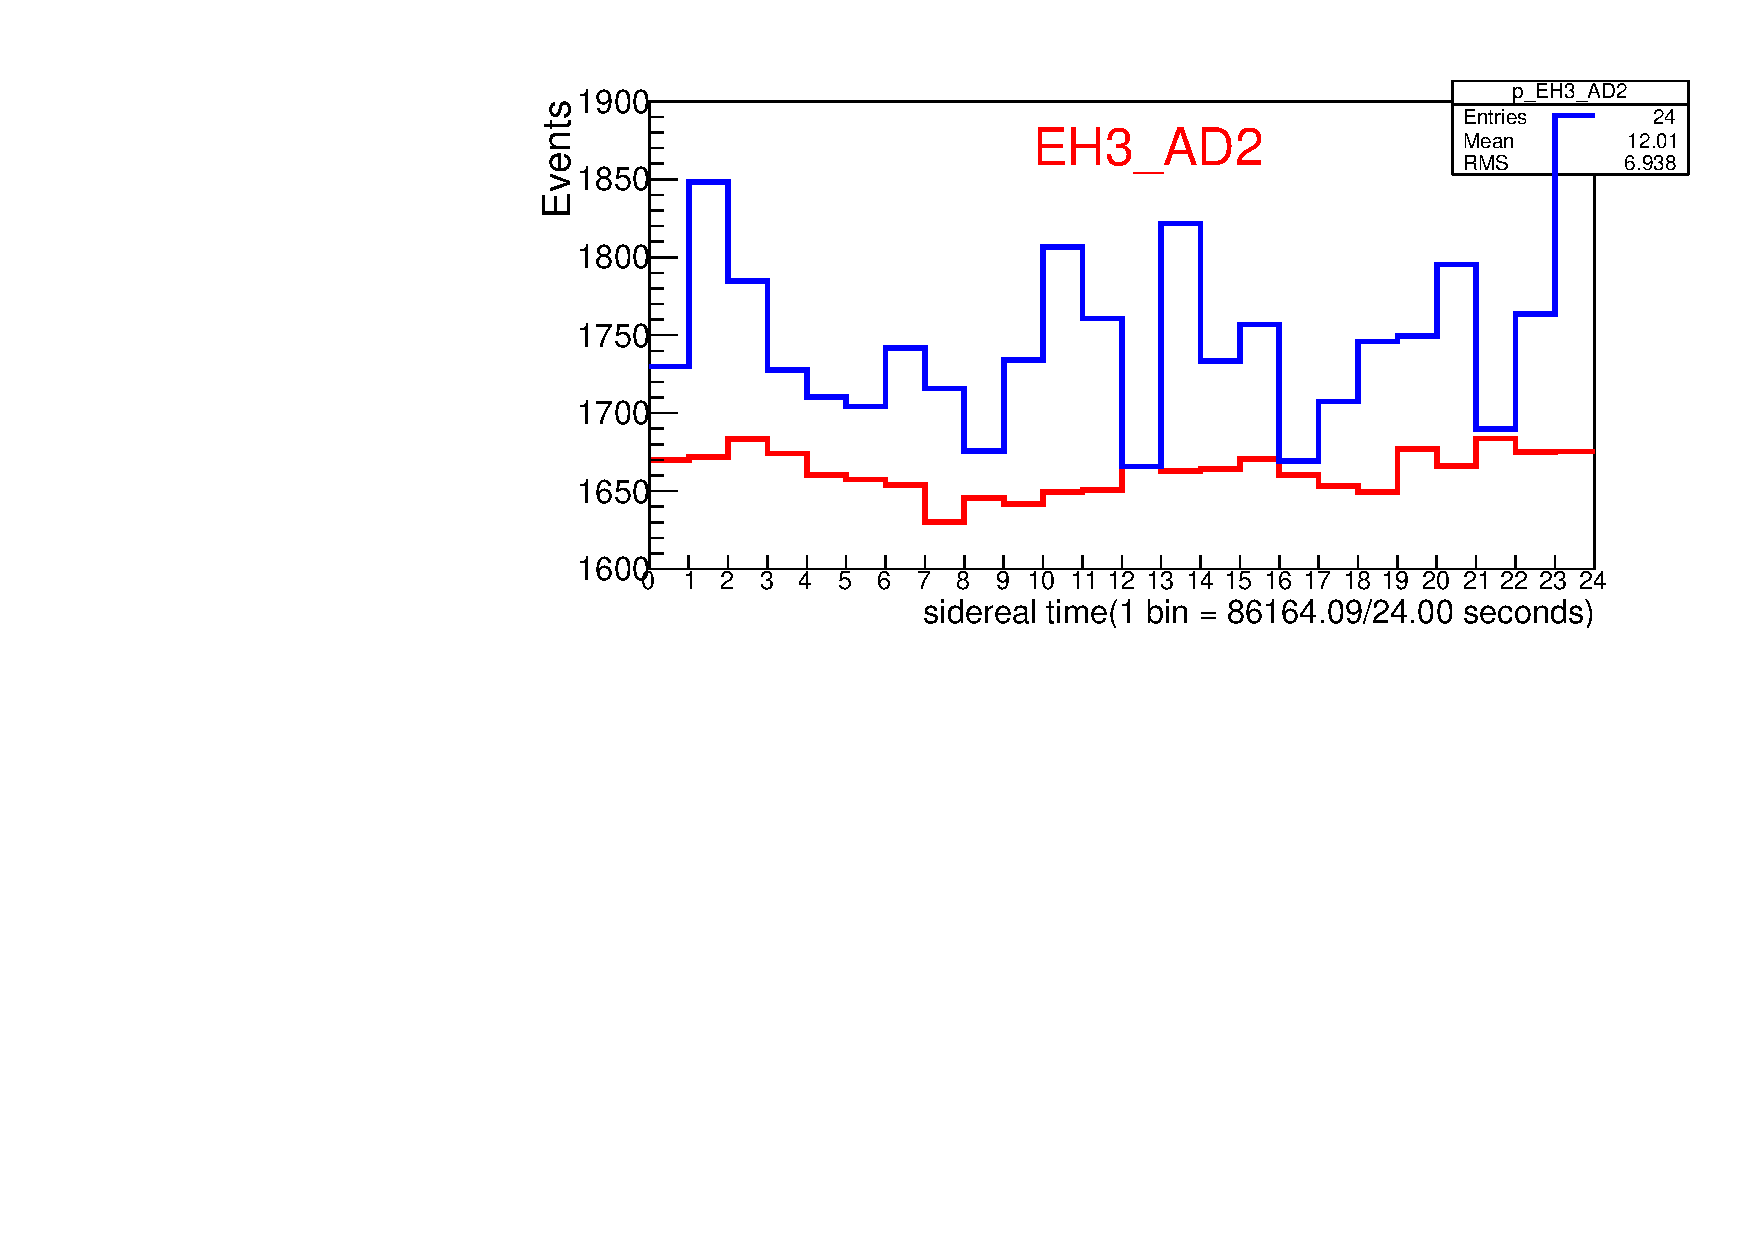
\includegraphics[width=6cm]{MeasurementPredictionEH3_AD2.pdf}\\
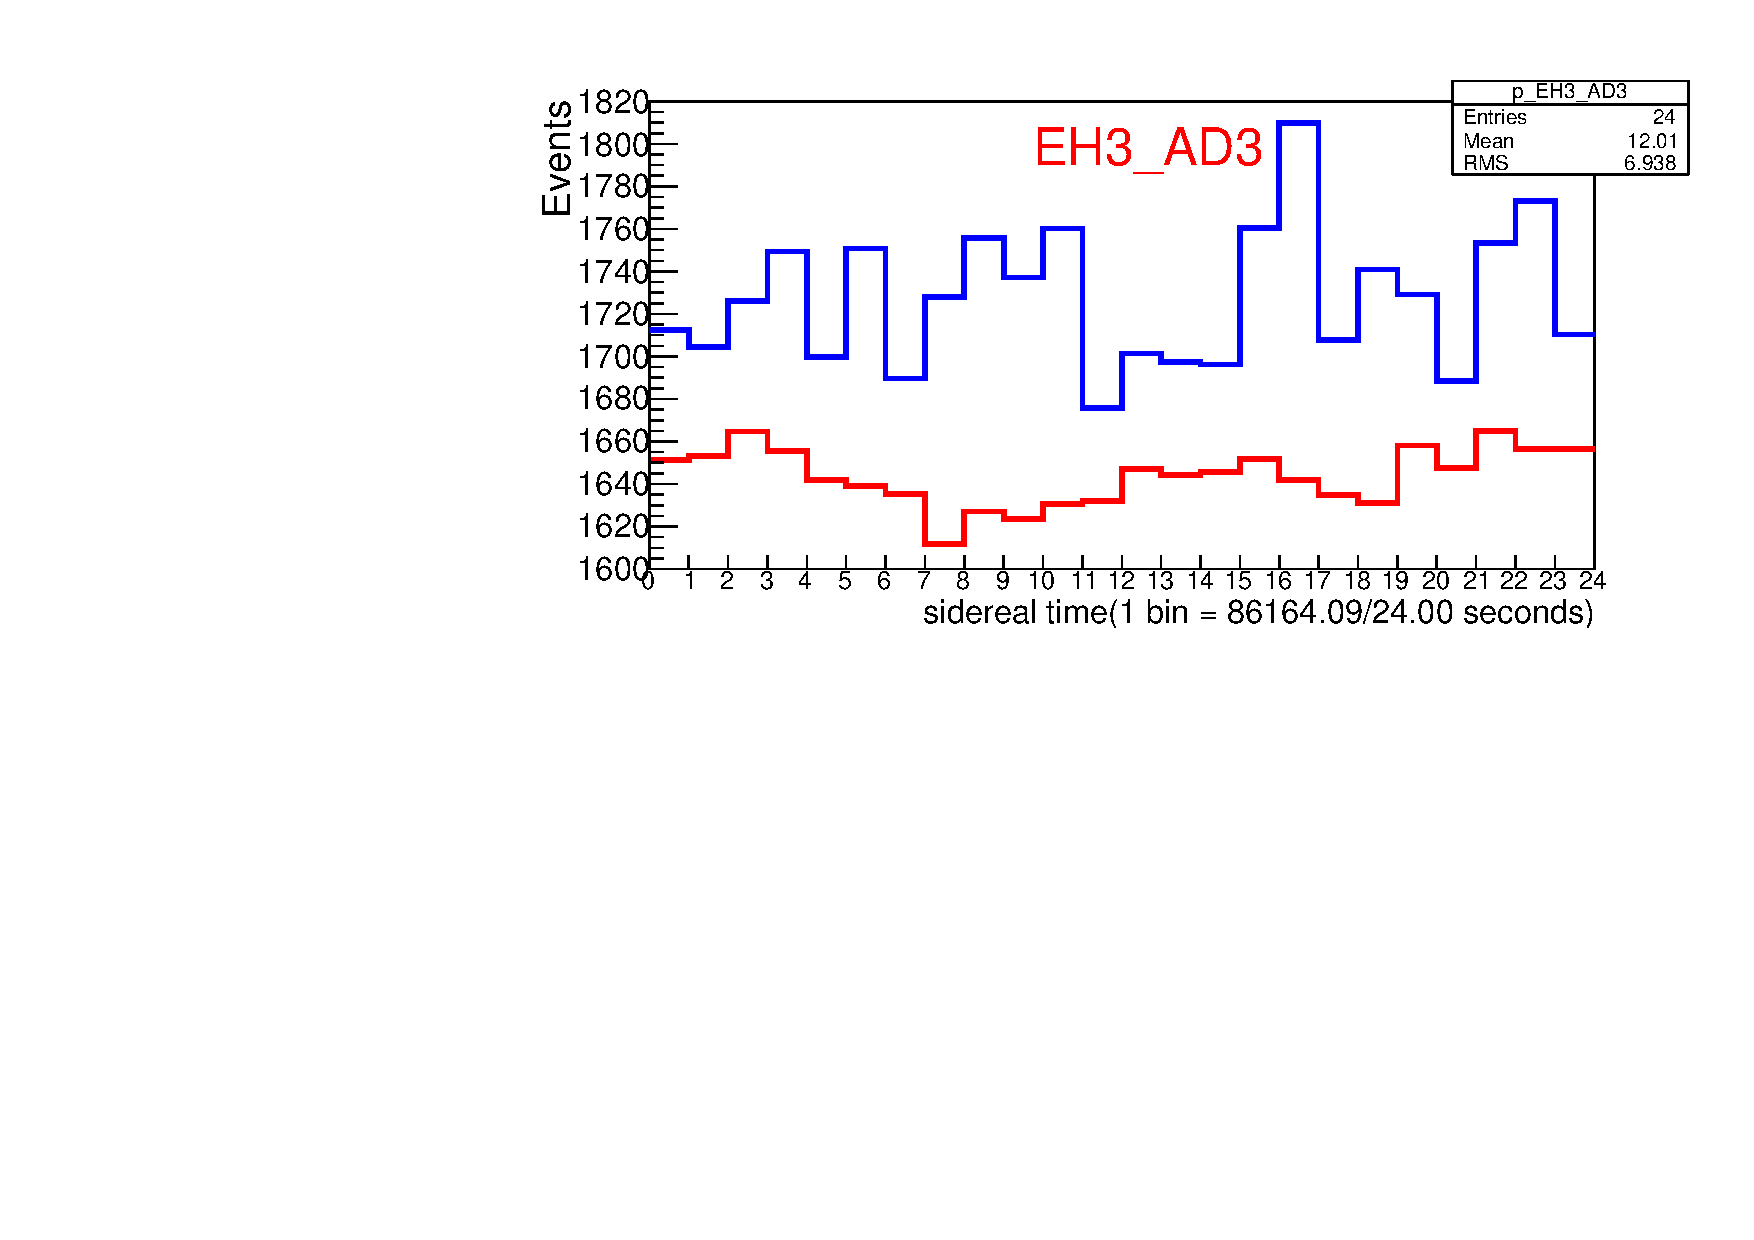
\includegraphics[width=6cm]{MeasurementPredictionEH3_AD3.pdf}
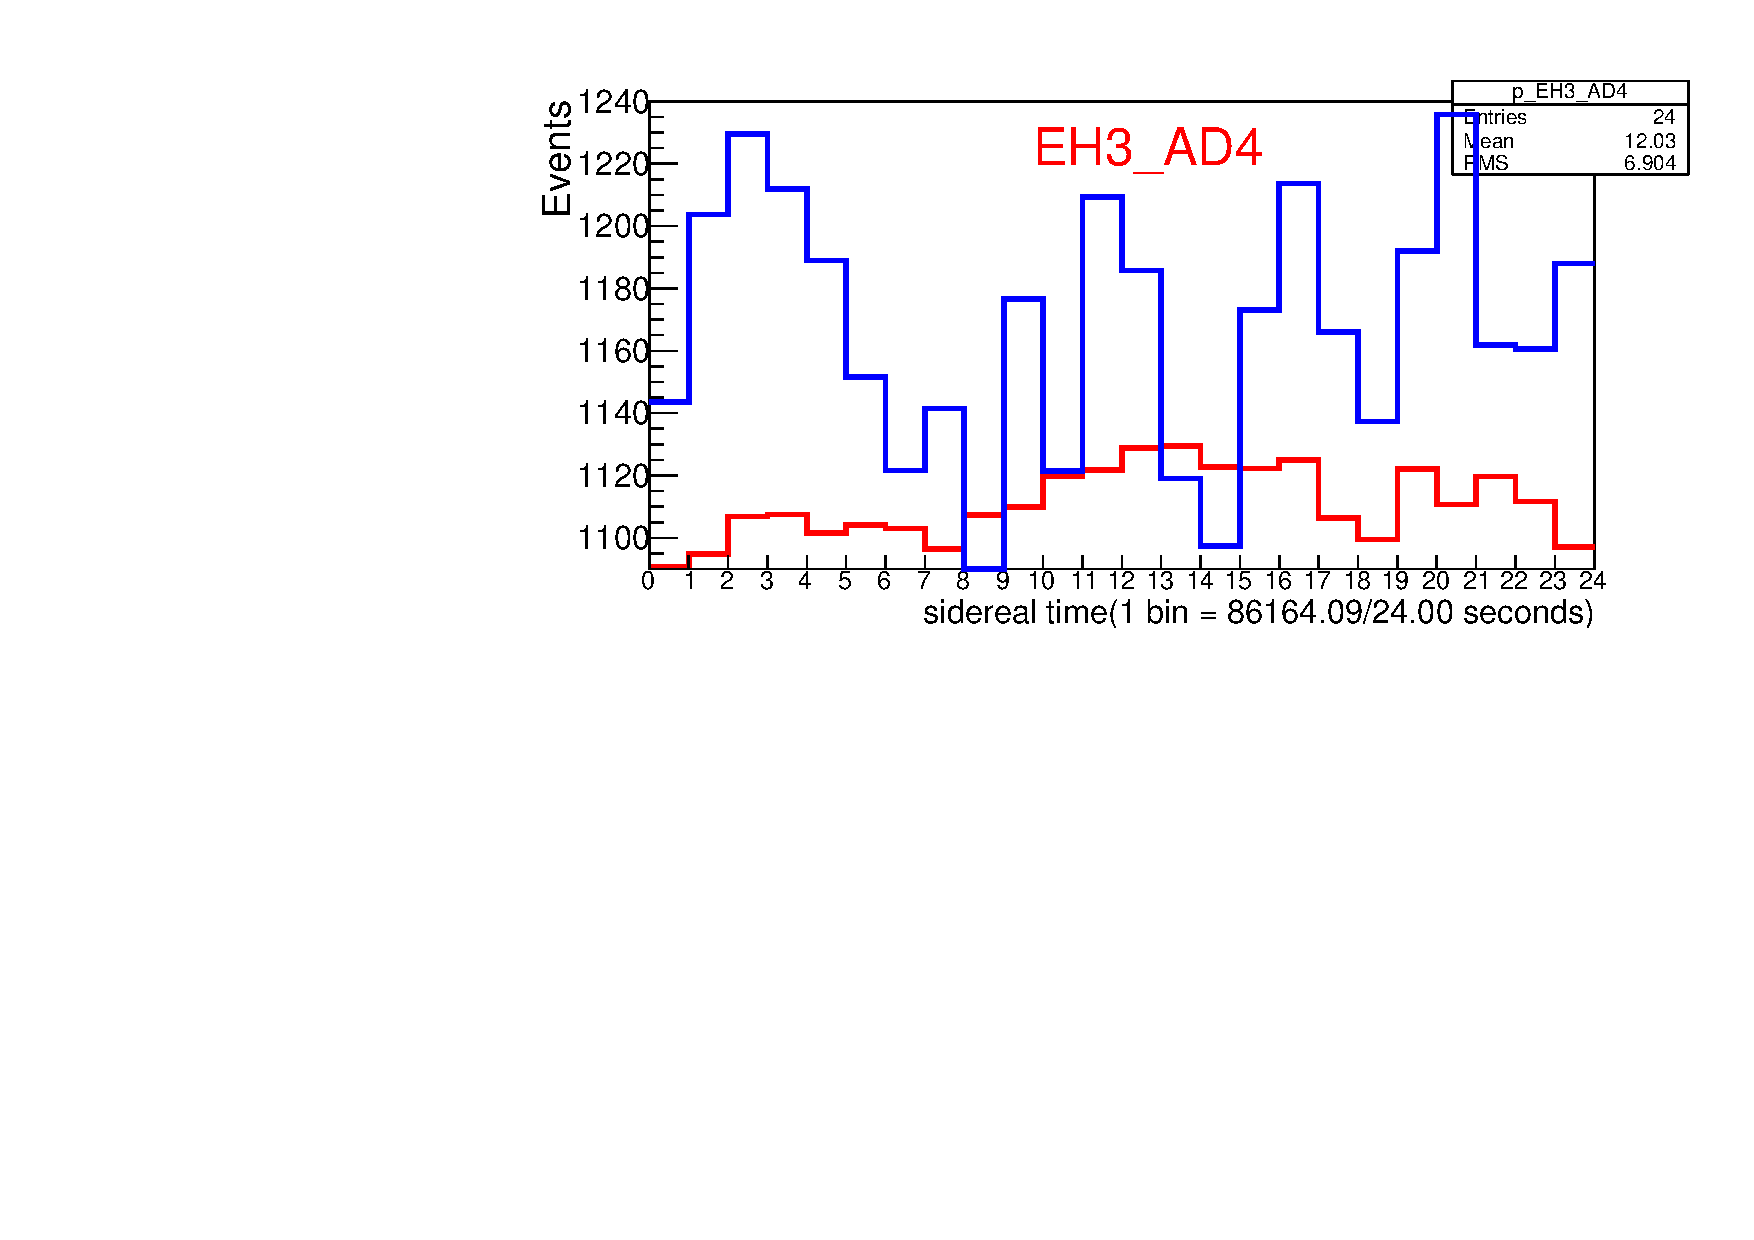
\includegraphics[width=6cm]{MeasurementPredictionEH3_AD4.pdf}
\caption{\textcolor{blue}{Measurement} and \textcolor{red}{Prediction} for each AD. The M/P ratio for each Hall is the weighted average of the ratio for each AD.} 
\end{center} 
\end{figure} 
 


\end{document}
